\subsection{Booting on x86 platforms}

\begin{frame}{Legacy BIOS booting (1)}
  \begin{itemize}
  \item x86 platforms shipped before 2005-2006 include a firmware
    called {\em BIOS}
    \begin{itemize}
    \item BIOS = Basic Input Output System
    \item Part of the hardware platform, closed-source, rarely
      modifiable
    \item Implements the booting process
    \item Provides runtime services that can be invoked - not commonly
      used
    \item Stored in some flash memory, outside of regular
      user-accessible storage devices
    \end{itemize}
  \item To be bootable, the first sector of a storage device is
    ``special''
    \begin{itemize}
    \item MBR = Master Boot Record
    \item Contains the partition table
    \item Contains up to 446 bytes of bootloader code, loaded into RAM
      and executed
    \item The BIOS is responsible for the RAM initialization
    \end{itemize}
  \item \url{https://en.wikipedia.org/wiki/BIOS}
  \end{itemize}
\end{frame}

\begin{frame}{Legacy BIOS booting (2)}
  \begin{itemize}
  \item Due to the limitation in size of the bootloader, bootloaders
    are split into two stages
    \begin{itemize}
    \item Stage 1, which fits within the 446 bytes constraint
    \item Stage 2, which is loaded by stage 1, and can therefore be
      bigger
    \end{itemize}
  \item Stage 2 is typically stored outside of any filesystem, at a
    fixed offset $\rightarrow$ simpler to load by stage 1
  \item Stage 2 generally has filesystem support, so it can load the
    kernel image from a filesystem
  \end{itemize}
\end{frame}

\begin{frame}{Legacy BIOS booting: sequence and storage}
  \begin{center}
    \includegraphics[width=0.7\textwidth]{slides/linux-bootloaders-sequence/legacy-bios-sequence.pdf}\\
    \vspace{0.5cm}
    \includegraphics[width=0.9\textwidth]{slides/linux-bootloaders-sequence/legacy-bios-storage.pdf}
  \end{center}
\end{frame}

\begin{frame}{UEFI booting}
  \begin{itemize}
  \item Starting from 2005-2006, UEFI is the new firmware interface on
    x86 platforms
    \begin{itemize}
    \item Unified Extensible Firmware Interface
    \item Describes the interface between the operating system and the
      firmware
    \item Firmware in charge of booting
    \item Firmware also provides runtime services to the operating
      system
    \item Stored in some flash memory, outside of regular
      user-accessible storage devices
    \end{itemize}
  \item Loads EFI binaries from the {\em EFI System Partition}
    \begin{itemize}
    \item Generally a bootloader
    \item Can also be directly the Linux kernel, with an {\em EFI Boot
        Stub}
    \end{itemize}
  \item Special partition, formatted with the {\em FAT} filesystem
    \begin{itemize}
    \item MBR: identified by type \code{0xEF}
    \item GPT: identified with a specific {\em globally unique identifier}
    \end{itemize}
  \item File \code{/efi/boot/bootx32.efi}, \code{/efi/boot/bootx64.efi}
  \item \url{https://en.wikipedia.org/wiki/UEFI}
  \end{itemize}
\end{frame}

\begin{frame}{UEFI booting: sequence and storage}
  \begin{center}
    \includegraphics[width=0.7\textwidth]{slides/linux-bootloaders-sequence/uefi-sequence.pdf}\\
    \vspace{0.5cm}
    \includegraphics[width=0.9\textwidth]{slides/linux-bootloaders-sequence/uefi-storage.pdf}
  \end{center}
\end{frame}

\begin{frame}{ACPI}
  \begin{itemize}
  \item Advanced Configuration and Power Interface
  \item {\em Open standard that operating systems can use to discover
      and configure computer hardware components, to perform power
      management, to perform auto configuration, and to perform status
      monitoring}
  \item {\em Tables} with descriptions of the hardware that cannot be
    dynamically discovered at runtime
  \item Tables provided by the firmware (UEFI or legacy) and used by
    the operating system (Linux kernel in our case)
  \item \small \url{https://en.wikipedia.org/wiki/Advanced_Configuration_and_Power_Interface}
  \end{itemize}
\end{frame}

\begin{frame}{UEFI and ACPI on ARM}
  \begin{itemize}
  \item Historically UEFI and ACPI are technologies coming from the
    Intel/x86 world
  \item ARM is also pushing for the adoption of UEFI and ACPI as part
    of its {\em ARM System Ready} certification
    \begin{itemize}
    \item Mainly for servers/workstations SoCs
    \item Does not impact embedded SoCs
    \item Currently not common in embedded Linux projects on ARM
    \item \url{https://www.arm.com/architecture/system-architectures/systemready-certification-program}
    \end{itemize}
  \item Also some on-going effort to use UEFI on RISC-V, but not the
    de-facto standard
  \item When an embedded platform uses UEFI $\rightarrow$ its booting
    process is similar to an {\em x86} platform
  \end{itemize}
\end{frame}

\subsection{Booting on embedded platforms}

\begin{frame}{Booting on embedded platforms: ROM code}
  \begin{itemize}
  \item Most embedded processors include a {\bf ROM code} that
    implements the initial step of the boot process
  \item The ROM code is written by the processor vendor and directly
    built into the processor
    \begin{itemize}
    \item Cannot be changed or updated
    \item Its behavior is described in the processor datasheet
    \end{itemize}
  \item Responsible for finding a suitable bootloader, loading it and
    running it
    \begin{itemize}
    \item From NAND/NOR flash, from USB, from SD card, from eMMC, etc.
    \item Well defined location/format
    \end{itemize}
  \item {\em Generally} runs with the external RAM not initialized, so
    it can only load the bootloader into an internal SRAM
    \begin{itemize}
    \item Limited size of the bootloader, due to the size of the SRAM
    \item Forces the boot process to be split in two steps: first
      stage bootloader (small, runs from SRAM, initializes external DRAM),
      second stage bootloader (larger, runs from external DRAM)
    \end{itemize}
  \end{itemize}
\end{frame}

\begin{frame}{Booting on STM32MP1: datasheet}
  \begin{columns}
    \column{0.7\textwidth}
    \begin{center}
      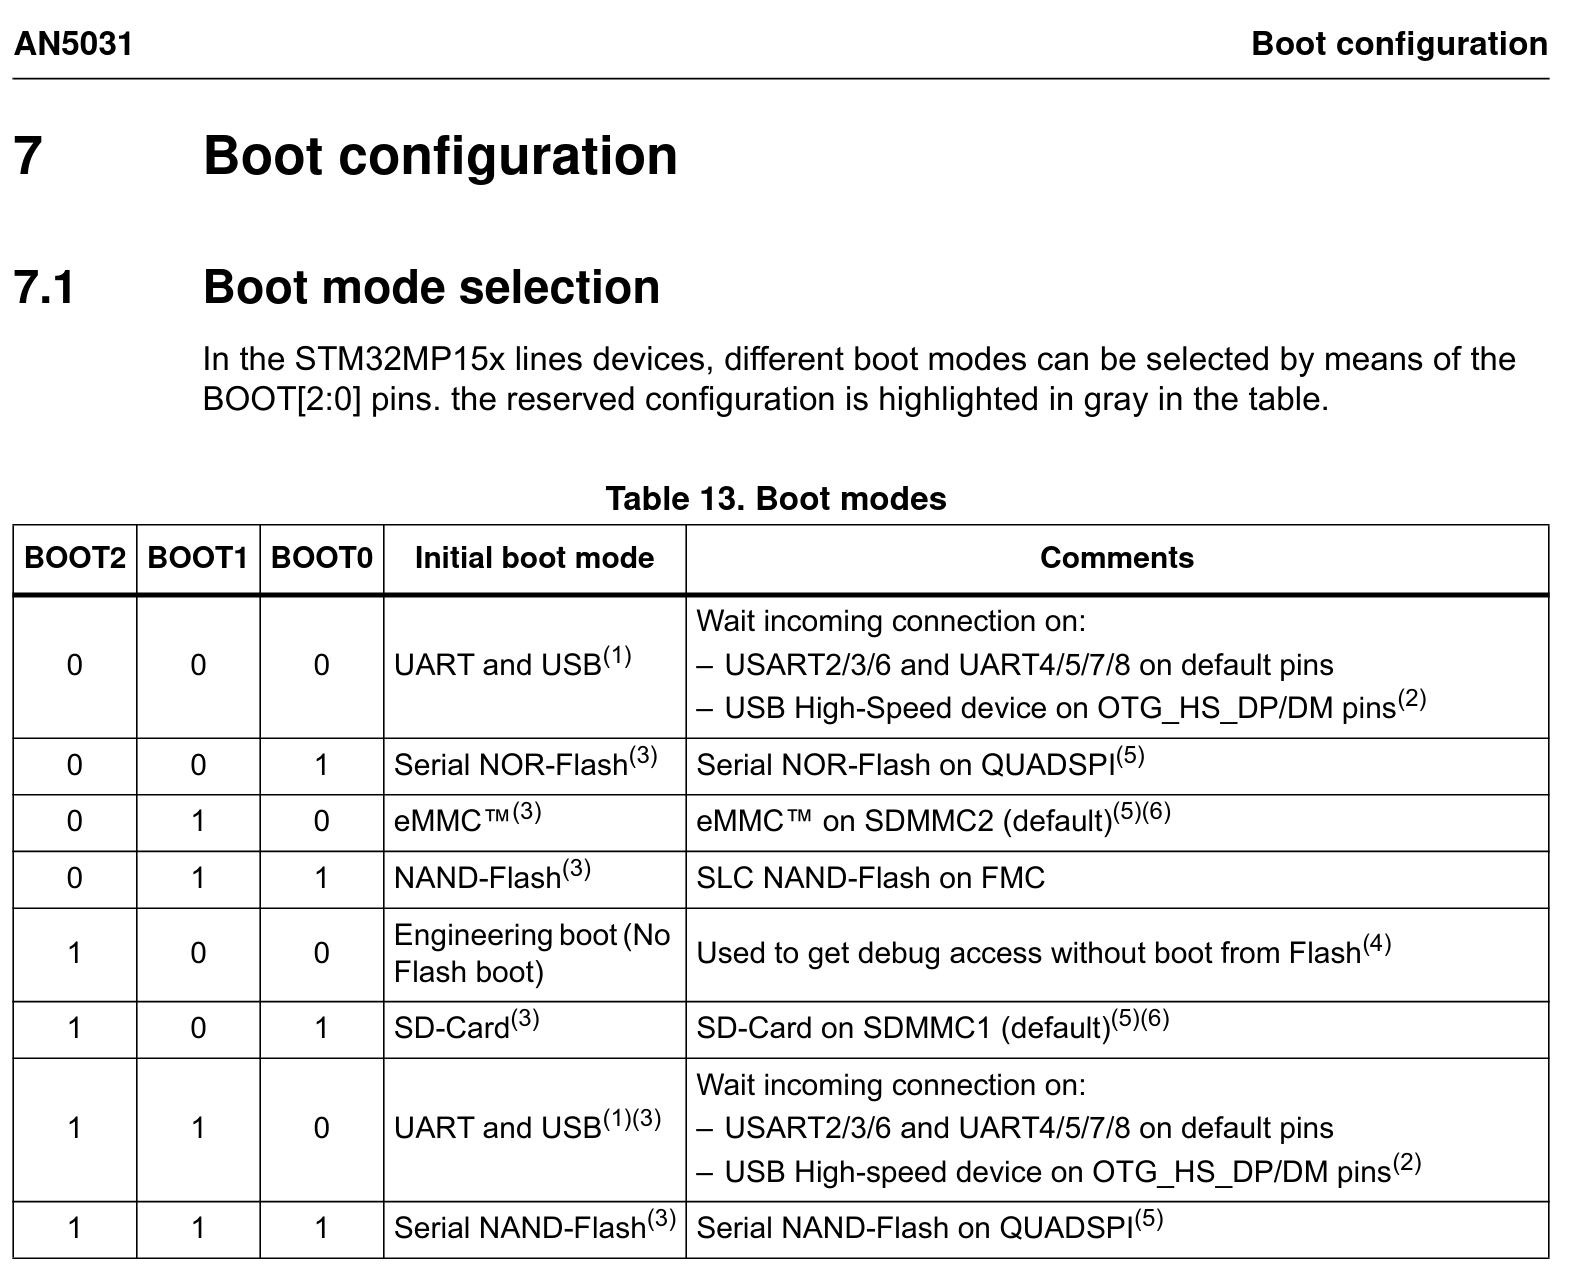
\includegraphics[height=0.84\textheight]{slides/linux-bootloaders-sequence/stm32mp1-rom-code.png}
    \end{center}
    \column{0.3\textwidth}
    {\tiny
      Source: \url{https://www.st.com/resource/en/application_note/dm00389996-getting-started-with-stm32mp151-stm32mp153-and-stm32mp157-line-hardware-development-stmicroelectronics.pdf}\\
      Useful details: \url{https://wiki.st.com/stm32mpu/wiki/STM32_MPU_ROM_code_overview}
    }
  \end{columns}
\end{frame}

\begin{frame}{Booting on AM335x (32 bit BeagleBone): datasheet}
  \begin{columns}
      \column{0.6\textwidth}
      \begin{center}
        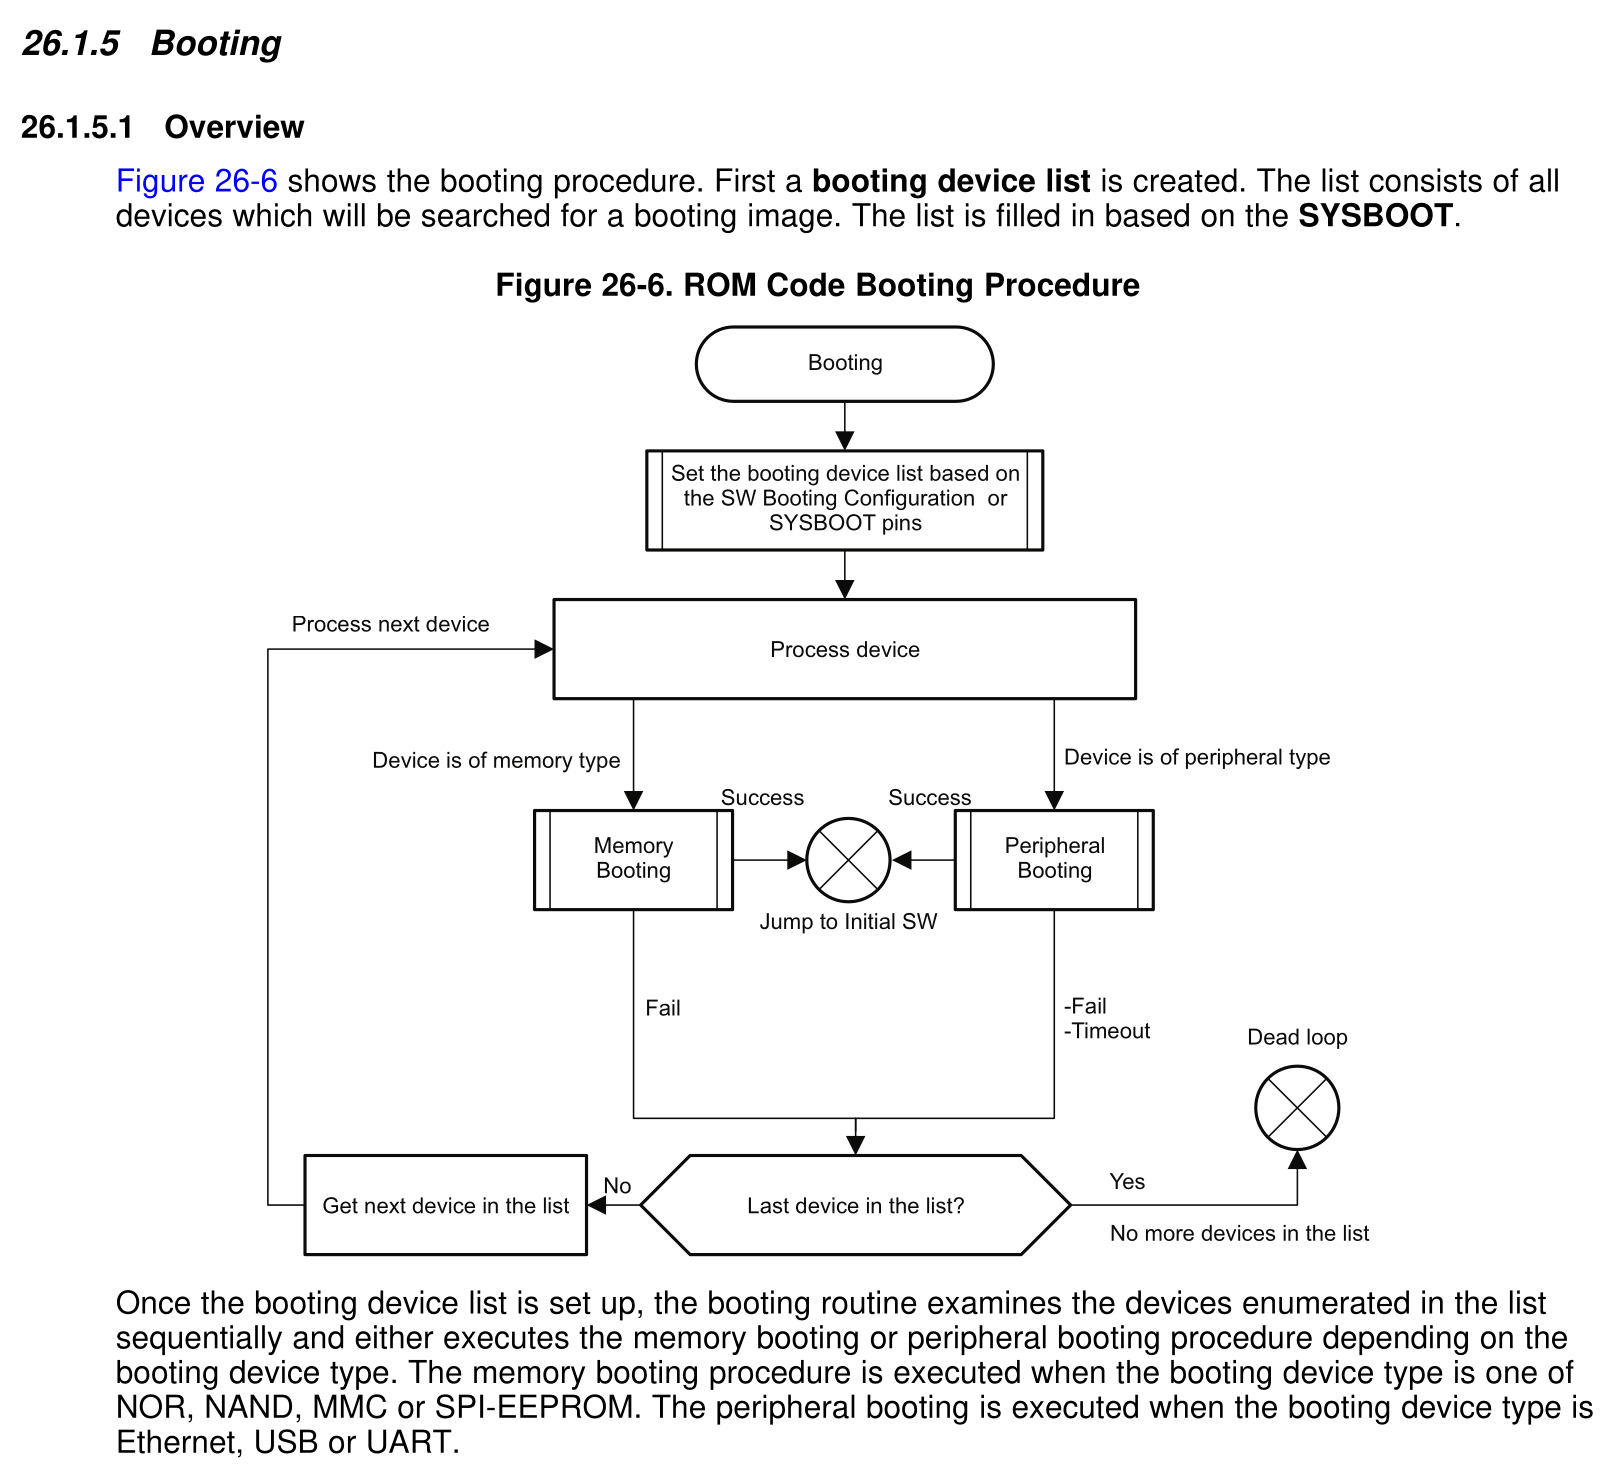
\includegraphics[height=0.84\textheight]{slides/linux-bootloaders-sequence/am335x-rom-code.png}
      \end{center}
      \column{0.4\textwidth}
      {\tiny
        Source:\\
        \url{https://www.mouser.com/pdfdocs/spruh73h.pdf},\\chapter 26
      }
    \end{columns}
\end{frame}

\begin{frame}{Two stage booting sequence}
  \begin{center}
    \includegraphics[height=0.85\textheight]{slides/linux-bootloaders-sequence/two-step-boot-process.pdf}
  \end{center}
\end{frame}

\begin{frame}{ROM code recovery mechanism}
  \begin{columns}
    \footnotesize
    \column{0.6\textwidth}
    \begin{itemize}
    \item Most ROM code also provide some sort of {\em recovery}
      mechanism, allowing to flash a board with no bootloader or a broken
      one, usually with a vendor-specific protocol over UART or USB.
    \item Often allows to push a new bootloader into RAM, making it
      possible to reflash the bootloader.
    \item Vendor-specific tools to run on the workstation
      \begin{itemize}
      \item STM32MP1: \href{https://www.st.com/en/development-tools/stm32cubeprog.html}{STM32 Cube Programmer}
      \item NXP i.MX: \href{https://github.com/NXPmicro/mfgtools}{uuu}
      \item Microchip AT91/SAM: \href{https://www.microchip.com/en-us/development-tool/SAM-BA-In-system-Programmer}{SAM-BA}
      \item Allwinner: \href{https://github.com/linux-sunxi/sunxi-tools}{sunxi-fel}
      \item Some open-source, some proprietary
      \end{itemize}
    \item Snagboot: new vendor agnostic tool replacing the above ones:
          \url{https://github.com/bootlin/snagboot}
    \end{itemize}
    \column{0.4\textwidth}
    \includegraphics[width=\textwidth]{slides/linux-bootloaders-sequence/stm32mp1-rom-code-recovery.pdf}
  \end{columns}
\end{frame}
